% fig16-followup-taxonomy.tex
% Paired follow-up intervention taxonomy on solved-baseline rows
\documentclass[tikz,border=18pt]{standalone}
% common-styles.tex
% Shared TikZ styles for wonton-proof paper figures

\usepackage{silence}
\WarningFilter{latex}{Missing character} 
\tracinglostchars=0 % Suppress engine-level "Missing character" warnings

\usepackage{fontspec}
\usepackage{unicode-math}

% Use filenames for reliability with Tectonic
\setmainfont{LibertinusSerif-Regular.otf}[
    BoldFont=LibertinusSerif-Bold.otf,
    ItalicFont=LibertinusSerif-Italic.otf,
    BoldItalicFont=LibertinusSerif-BoldItalic.otf
]
\setsansfont{LibertinusSans-Regular.otf}[
    BoldFont=LibertinusSans-Bold.otf,
    ItalicFont=LibertinusSans-Italic.otf
]
\setmonofont{LibertinusMono-Regular.otf}

% Try a more standard math font if LibertinusMath is causing nullfont issues
\setmathfont{LibertinusMath-Regular.otf}
% \setmathfont{latinmodern-math.otf}[range=digits] 

\usepackage{amsmath}
\usepackage{tikz}
\usepackage{forest}

\usetikzlibrary{
    arrows.meta,
    calc,
    decorations.pathreplacing,
    fit,
    positioning,
    shapes.geometric,
    shapes.misc,
    backgrounds,
    shadows.blur,
    fadings
}

% Color palette (muted, print-friendly)
\definecolor{ink}{RGB}{45,45,52}
\definecolor{muted}{RGB}{115,115,125}
\definecolor{highlight}{RGB}{198,120,44}
\definecolor{accentblue}{RGB}{86,130,178}
\definecolor{accentgreen}{RGB}{84,156,132}
\definecolor{blocked}{RGB}{140,75,75}
\definecolor{goalnode}{RGB}{255,255,255}
\definecolor{terminal}{RGB}{238,239,244}
\definecolor{deadnode}{RGB}{248,245,245}
\definecolor{flowbox}{RGB}{250,250,252}
\definecolor{basin1}{RGB}{224,234,248}
\definecolor{basin2}{RGB}{246,232,221}
\definecolor{basin3}{RGB}{228,242,234}
\definecolor{heatbase}{RGB}{86,130,178}

\tikzset{
    line cap=round,
    line join=round,
    pop/.style={
        blur shadow={shadow blur steps=5, shadow blur extra rounding=1.3pt}
    },
    base node/.style={
        rounded rectangle,
        draw=ink,
        line width=0.6pt,
        fill=goalnode,
        text=ink,
        minimum width=2.2cm,
        minimum height=0.7cm,
        align=center,
        pop
    },
    goal/.style={base node, fill=goalnode},
    terminal/.style={base node, fill=terminal, line width=0.9pt},
    dead/.style={base node, fill=deadnode, dashed},
    flowbox/.style={
        rectangle,
        draw=muted,
        rounded corners=3pt,
        fill=flowbox,
        minimum width=1.8cm,
        minimum height=0.6cm,
        align=center,
        font=\normalfont\small,
        text=ink,
        pop
    },
    decision/.style={
        diamond,
        draw=muted,
        fill=flowbox,
        aspect=2.4,
        font=\normalfont\small,
        inner sep=1pt,
        text=ink
    },
    protocolbox/.style={
        rectangle,
        draw=muted,
        rounded corners=4pt,
        fill=flowbox,
        minimum width=2cm,
        minimum height=0.8cm,
        font=\normalfont\small,
        align=center,
        text=ink
    },
    tactic/.style={
        ->,
        >=Stealth,
        draw=muted,
        line width=0.75pt
    },
    tacticlight/.style={
        ->,
        >=Stealth,
        draw=muted!45,
        dashed,
        line width=0.6pt
    },
    backprop/.style={
        ->,
        >=Stealth,
        draw=muted!70,
        dashed,
        line width=0.6pt
    },
    selected/.style={
        tactic,
        draw=highlight,
        line width=1.4pt
    },
    divergetactic/.style={
        tactic,
        draw=highlight,
        line width=1.4pt
    },
    divergenode/.style={
        base node,
        draw=highlight,
        line width=1.0pt
    },
    divergeblock/.style={
        blockedtactic,
        line width=1.2pt
    },
    blockedtactic/.style={
        tactic,
        draw=blocked,
        densely dashed
    },
    flowarrow/.style={
        ->,
        >=Stealth,
        draw=muted,
        line width=0.75pt
    },
    crosslink/.style={
        -,
        draw=muted!70,
        dotted,
        line width=0.6pt
    },
    annot/.style={
        font=\normalfont\footnotesize,
        text=muted
    },
    visit/.style={
        annot,
        font=\normalfont\scriptsize
    },
    annotbg/.style={
        annot,
        fill=white,
        inner sep=1.5pt
    },
    tacticlabel/.style={
        annot,
        font=\ttfamily\footnotesize,
        text=muted
    },
    formula/.style={
        font=\normalfont\footnotesize,
        draw=muted,
        rounded corners=2pt,
        fill=white,
        inner sep=3pt
    },
    paneltitle/.style={
        font=\normalfont\bfseries,
        text=ink
    },
    trajectory/.style={
        ->,
        draw=muted!70,
        line width=0.6pt
    }
}


\begin{document}
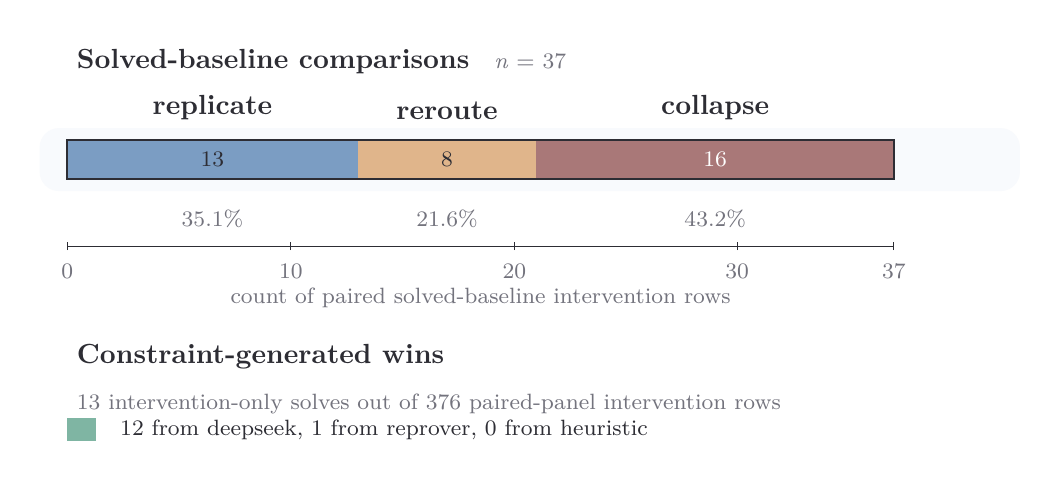
\begin{tikzpicture}[
    every node/.style={font=\small},
    show background rectangle,
    background rectangle/.style={fill=white}
]

\def\maxw{10.5}
\def\repw{3.69}   % 13 / 37
\def\rerw{2.27}   % 8 / 37
\def\colw{4.54}   % 16 / 37

\node[paneltitle, anchor=west] at (0, 4.55) {Solved-baseline comparisons};
\node[annot, anchor=west] at (5.3, 4.55) {\textit{n} = 37};

\path[fill=basin1!24, rounded corners=7pt] (-0.35, 2.9) rectangle (\maxw + 1.6, 3.7);
\fill[accentblue!78] (0, 3.05) rectangle (\repw, 3.55);
\fill[highlight!55] (\repw, 3.05) rectangle (\repw + \rerw, 3.55);
\fill[blocked!75] (\repw + \rerw, 3.05) rectangle (\maxw, 3.55);
\draw[ink, line width=0.6pt] (0, 3.05) rectangle (\maxw, 3.55);

\node[paneltitle, text=ink, anchor=south] at (\repw/2, 3.68) {replicate};
\node[paneltitle, text=ink, anchor=south] at (\repw + \rerw/2, 3.68) {reroute};
\node[paneltitle, text=ink, anchor=south] at (\repw + \rerw + \colw/2, 3.68) {collapse};

\node[annot, text=ink] at (\repw/2, 3.3) {13};
\node[annot, text=ink] at (\repw + \rerw/2, 3.3) {8};
\node[annot, text=white] at (\repw + \rerw + \colw/2, 3.3) {16};

\node[annot, anchor=north] at (\repw/2, 2.78) {35.1\%};
\node[annot, anchor=north] at (\repw + \rerw/2, 2.78) {21.6\%};
\node[annot, anchor=north] at (\repw + \rerw + \colw/2, 2.78) {43.2\%};

\draw[ink, line width=0.5pt] (0, 2.2) -- (\maxw, 2.2);
\foreach \x/\label in {0/0, 2.84/10, 5.68/20, 8.51/30, 10.5/37} {
    \draw[ink, line width=0.4pt] (\x, 2.15) -- (\x, 2.25);
    \node[annot, anchor=north] at (\x, 2.1) {\label};
}
\node[annot] at (5.25, 1.55) {count of paired solved-baseline intervention rows};

\node[paneltitle, anchor=west] at (0, 0.8) {Constraint-generated wins};
\node[annot, anchor=north west, align=left] at (0, 0.45) {13 intervention-only solves out of 376 paired-panel intervention rows};
\fill[accentgreen!75] (0, -0.28) rectangle (0.36, 0.02);
\node[annot, anchor=west, text=ink] at (0.55, -0.13) {12 from deepseek, 1 from reprover, 0 from heuristic};

\end{tikzpicture}
\end{document}
